\documentclass{article}

\usepackage{arxiv}

\usepackage[utf8]{inputenc} % allow utf-8 input
\usepackage[T1]{fontenc}    % use 8-bit T1 fonts
\usepackage[hidelinks]{hyperref}       % hyperlinks
\usepackage{url}            % simple URL typesetting
\usepackage{booktabs}       % professional-quality tables
\usepackage{amsmath,amssymb,amsthm}
\usepackage{amsfonts}       % blackboard math symbols
\usepackage{nicefrac}       % compact symbols for 1/2, etc.
\usepackage{makecell}
\usepackage{microtype}      % microtypography
\usepackage{mathrsfs}
\usepackage{graphicx}
\usepackage{doi}
\usepackage{acronym}
\usepackage{listings}
\usepackage{tikz}
\usepackage[dvipsnames]{xcolor}

\usetikzlibrary{trees}

\def\checkmark{\tikz\fill[scale=0.4](0,.35) -- (.25,0) -- (1,.7) -- (.25,.15) -- cycle;}
\def\cross{\tikz\draw[scale=0.3, black, line width=0.3mm](0,0) -- (1,1) -- (0.5,0.5) -- (0,1) -- (1,0) -- (0.5,0.5);}

\newacro{abm}[ABM]{Agent-Based Model}
\newacro{cabm}[CABM]{Cellular Agent-Based Model}
\newacro{ca}[CA]{Cellular Automaton}
\newacro{ib}[IB]{Individual-Based}
\newacroplural{ca}[CA]{Cellular Automata}

\newcommand{\todo}[1]{\colorbox{WildStrawberry}{\textcolor{white}{#1}}}

\newcommand{\R}{\mathbb{R}}

\title{
    Mathematical Foundations of\\
    Cellular Agent-Based Models
}

%\date{September 9, 1985}	% Here you can change the date presented in the paper title
%\date{} 					% Or removing it

\author{
    \href{https://orcid.org/0009-0001-0613-7978}{
        
\includegraphics[scale=0.06]{orcid.pdf}
        \hspace{1mm}Jonas Pleyer
    }
    \thanks{
        \href{https://jonas.pleyer.org}{jonas.pleyer.org},
        \href{https://cellular-raza.com}{cellular-raza.com}
    }\\
	Freiburg Center for Data-Analysis and Modeling\\
	University of Freiburg\\
	\texttt{jonas.pleyer@fdm.uni-freiburg.de} \\
	%% examples of more authors
	\And
	\href{https://orcid.org/0000-0002-6371-4495}{
        
\includegraphics[scale=0.06]{orcid.pdf}
        \hspace{1mm}Christian Fleck
    }\\
	Freiburg Center for Data-Analysis and Modeling\\
	University of Freiburg
}

% Uncomment to remove the date
%\date{}

% Uncomment to override  the `A preprint' in the header
\renewcommand{\headeright}{Preprint}
%\renewcommand{\undertitle}{Technical Report}
\renewcommand{\shorttitle}{Mathematical Foundations of Cellular Agent-Based Models}

\usepackage{enumitem}
\setlist{nolistsep}

%%% Add PDF metadata to help others organize their library
%%% Once the PDF is generated, you can check the metadata with
%%% $ pdfinfo template.pdf
\hypersetup{
pdftitle={Mathematical Foundations of Cellular Agent-Based Models},
pdfsubject={q-bio.NC, q-bio.QM},
pdfauthor={Jonas Pleyer, Christian Fleck},
pdfkeywords={},
}

% Define definition, example, lemma, proof and theorem.
\newtheorem{definition}{Definition}[section]
\newtheorem{example}[definition]{Example}
\newtheorem{lemma}[definition]{Lemma}
\newtheorem{corollary}[definition]{Corollary}
\newtheorem{theorem}[definition]{Theorem}

% Change numbering of equations
% \numberwithin{equation}{section}

% MAKE TITLES IN THEOREMS BOLD
\makeatletter
\def\th@plain{%
  \thm@notefont{}% same as heading font
  \itshape % body font
}
\def\th@definition{%
  \thm@notefont{}% same as heading font
  \normalfont % body font
}
\makeatother

\begin{document}
\maketitle

%###################################################################################################
\begin{abstract}
    In this work, we lay out fundamental theoretical concepts of \ac{ib} \acp{abm} and argue why
    classical \acp{ca} should not generally be considered \ac{ib} \acp{abm}.
    We show that these concepts can encapsulate a wide class of available numerical simulation tools
    Furthermore, we present precise mathematical formulations of widely used examples such as
    cell-sorting and cell-cell communication.
    Extending our theoretical work, we discuss the process of spatial and remporal coarse-graining.
\end{abstract}
\vfill

% TABLE OF CONTENTS
% Remove this before submission
\pagebreak
\tableofcontents
\vfill
\pagebreak

% keywords can be removed
\keywords{Individual-Based \and Cell \and Biology \and Dynamical System}

\section{Introduction}
\section{Theoretical Framework}

\begin{itemize}
    \item Start listing aspects of cellular systems
    \item group aspects in table in (C) Cellular, (CC) Cell-Cell, (DC) Domain-Cell
    \item Concept figure to distinction of these aspect groups
    \item Discuss variations of these aspects on a conceptual level
    \item Discuss underlying assumptions: spatial locality, individual-based behaviour leads to
        collective effects
\end{itemize}

\begin{figure}
    \centering
    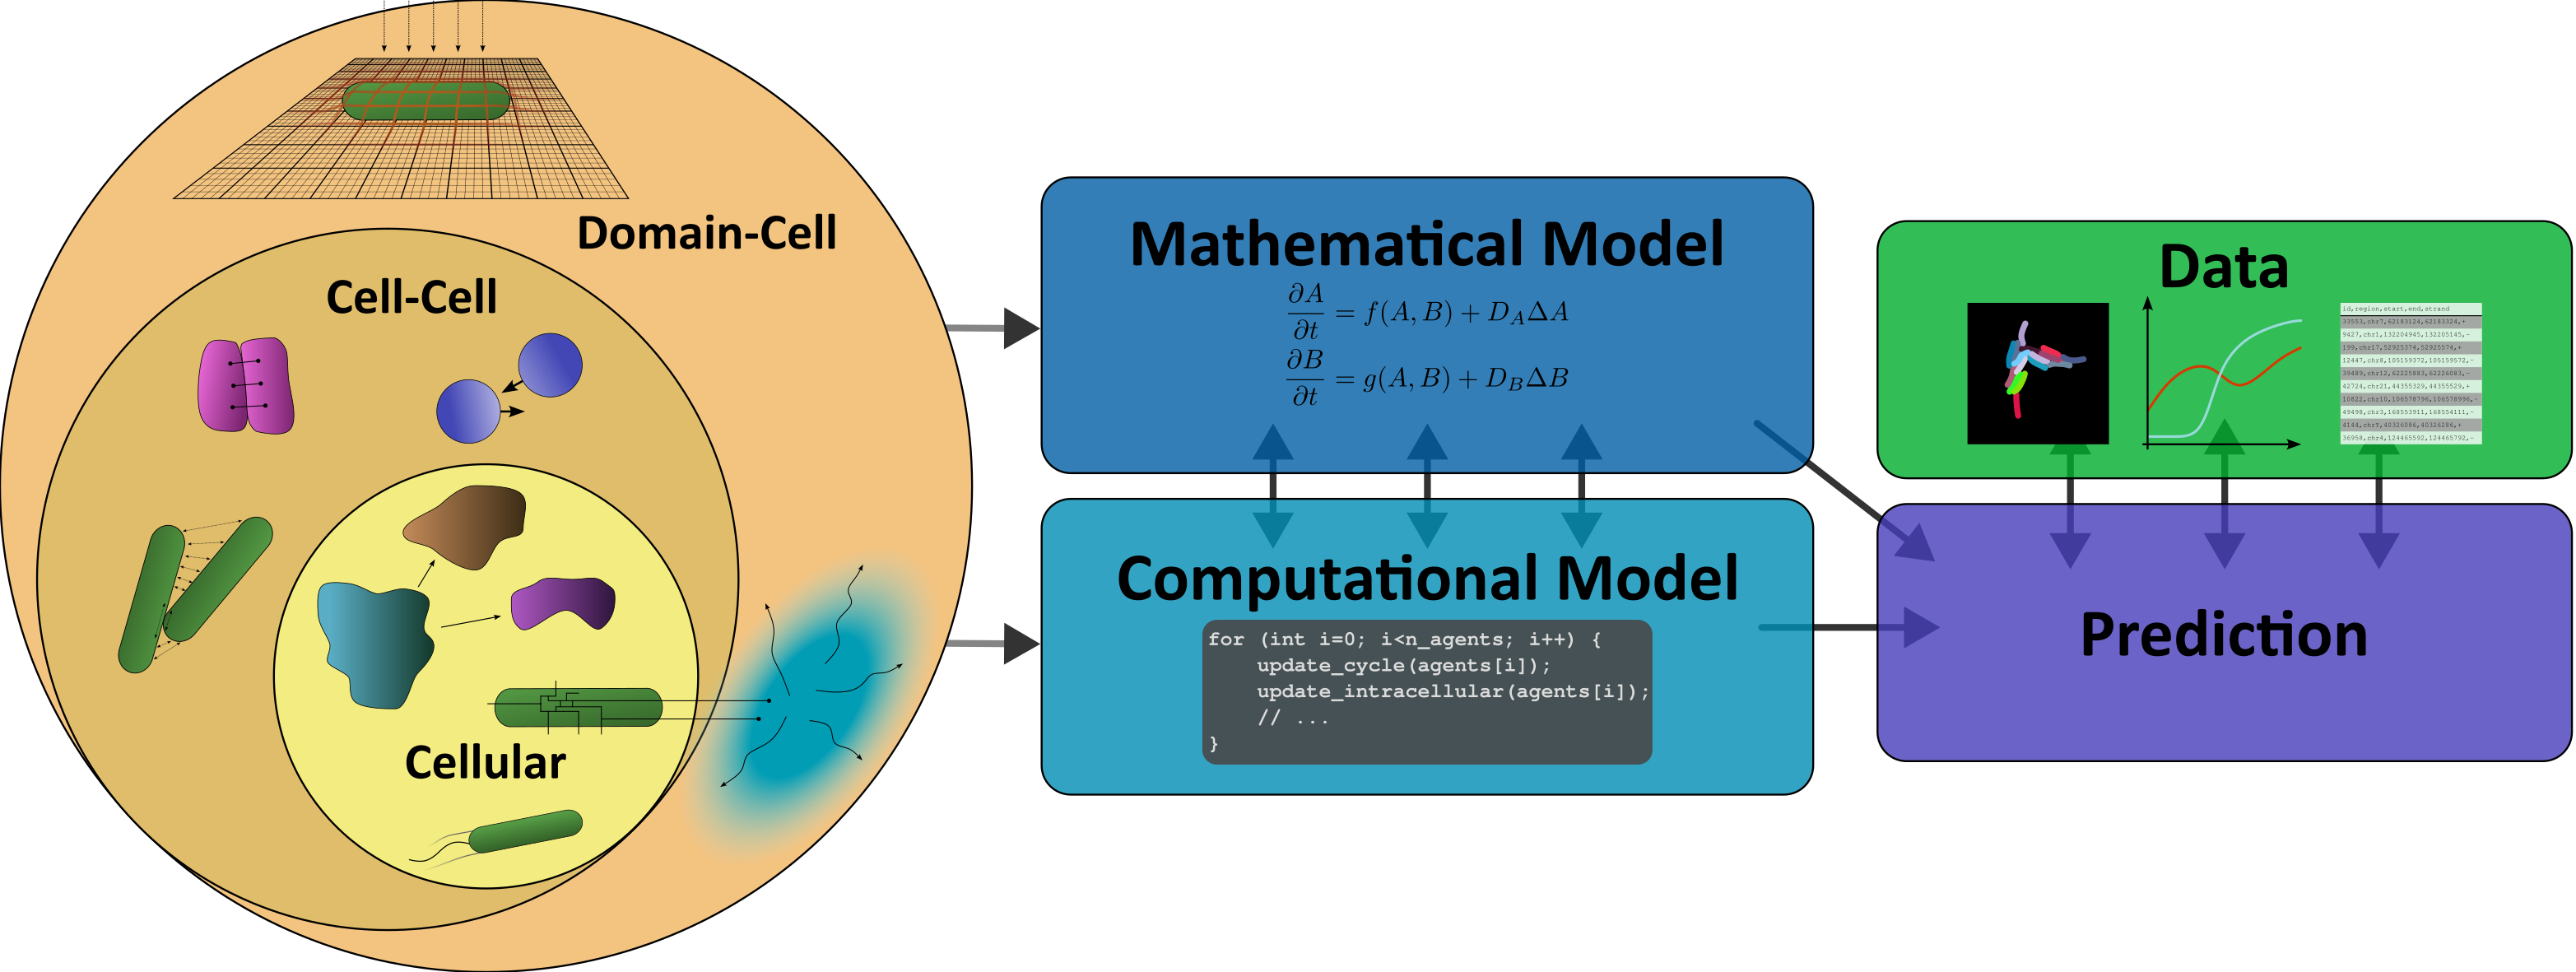
\includegraphics[width=\textwidth]{figures/concept-figure.png}
\end{figure}

\section{Parameter Estimation \& Sensitivity Analysis}
\section{Coarse-Graining \& Pattern Formation}

\subsection{Branching Patterns of \textit{Bacillus Subtilis}}

\begin{itemize}
    \item PDE models of bacterial branching \cite{Kawasaki1997,Matsushita1998}
\end{itemize}

\subsection{Cell Sorting}

\subsection{More Ideas}

\begin{itemize}
    \item \cite{Volfson2008} TODO; continuum model, equations of nematodynamics \cite{Doi1988-ad}
    \item \cite{Joshi2019} "The interplay between activity and filament flexibility determines the
        emergent properties of active nematics"
    \item \cite{Jin2020} "Influence of cell interaction forces on growth of bacterial biofilms"
    \item \cite{Ingham2008} "Swarming and complex pattern formation in Paenibacillus vortex studied
        by imaging and tracking cells"
\end{itemize}

\bibliographystyle{IEEEtran}
\bibliography{references}

\renewcommand{\thesection}{}
\renewcommand{\thesubsection}{S\arabic{subsection}}

\section{Supplementary Material}
\subsection{Elementary CA}

\end{document}
